\section{Phenix Dock in Map protocol}
\label{app:dockInMapProtocol}%a160
Protocol designed to automatically fit atomic structures to electron density maps in \scipion by using \phenix \ttt{dock in map} (\citep{Liebschner2019}), application that uses a convolution-based shape search with which it finds the parts of the \iii{map} that are similar to the \iii{model}. Additional information can be found in \url{http://www.phenix-online.org/documentation/reference/dock_in_map.html}.
   
 \begin{itemize}
  \item Requirements to run this protocol and visualize results:
    \begin{itemize}
        \item \scipion plugin: \ttt{scipion-em}
        \item \scipion plugin: \ttt{scipion-em-phenix}
        \item \phenix package (version 1.18)
        \item \scipion plugin: \ttt{scipion-em-chimera}
    \end{itemize}
  \item \scipion menu:\\
   \ttt{Model building -> Rigid fitting} (\ffigure{fig:app_protocol_dockInMap_1} (A))
  
  \item Protocol form parameters (\ffigure{fig:app_protocol_dockInMap_1} (B)):
  
    \begin{figure}[H]
     \centering 
     \captionsetup{width=.7\linewidth} 
     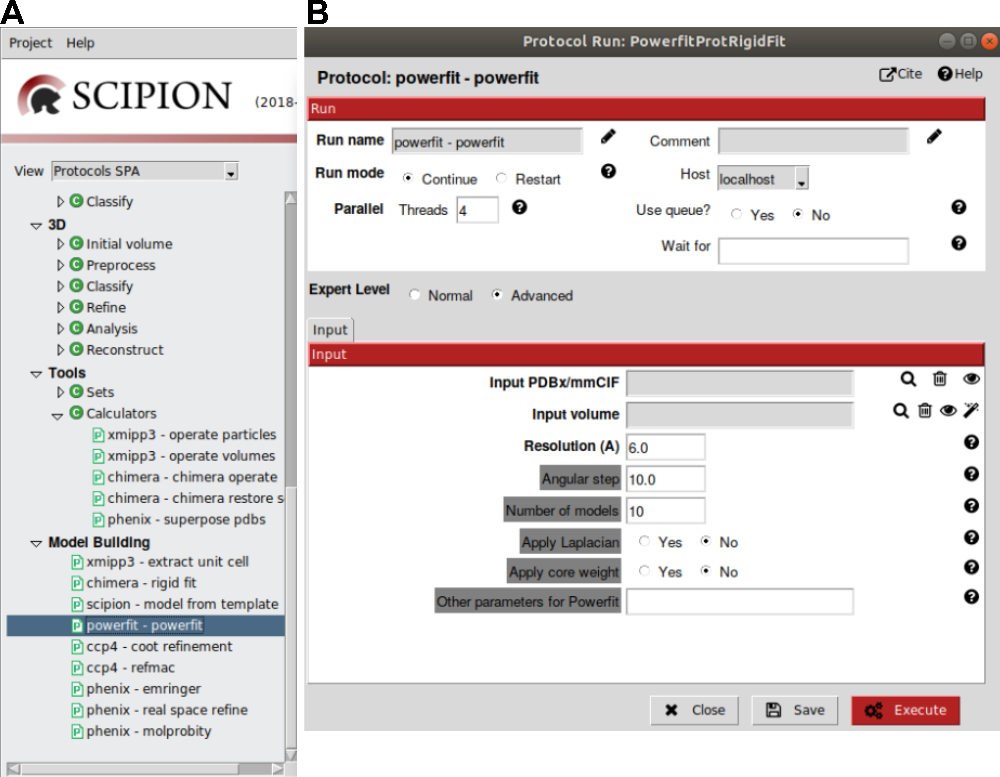
\includegraphics[width=0.90\textwidth]{Images_appendix/Fig113.pdf}
     \caption{Protocol \scommand{phenix - dock in map}. A: Protocol location in \scipion menu. B: Protocol form.}
     \label{fig:app_protocol_dockInMap_1}
    \end{figure}

    \begin{itemize}
     \item \ttt{Input map}: Electron density map previously downloaded or generated in \scipion to fit the atomic structure.
     \item \ttt{Resolution (\AA)}: Electron density map resolution.
     \item \ttt{Input atom structure}: Atomic structure previously downloaded or generated in \scipion to be fitted to an electron density map.
     \item \ttt{Atom structure number of copies}: Number of \iii{models} that have to be simultaneously fitted to an electron density map.
     \item \ttt{Number of threads}: Advanced param. Depending on the size of \iii{map} and \iii{model}, and the number of \iii{models} to fit the process could be quite slow and you can accelerate it by increasing the number of threads.
    \end{itemize}

  \item Protocol execution:
  
  Adding specific protocol label is recommended in \ttt{Run name} section, at the form top. To add the label, open the protocol form, press the pencil symbol at the right side of \ttt{Run name} box, complete the label in the new opened window, press OK and, finally, close the protocol. This label will be shown in the output summary content (see below). If you want to run again this protocol, do not forget to set to \ttt{Restart} the \ttt{Run mode}.\\
  Press the \ttt{Execute} red button at the form bottom.
  
  \item Visualization of protocol results:
  
  After executing the protocol, press \ttt{Analyze Results} and the \chimera graphics window will be opened by default. Atomic structures and volumes are referred to the origin of coordinates in \chimera. To show the relative position of atomic structure and electron density volume, the three coordinate axes are represented; X axis (red), Y axis (yellow), and Z axis (blue) (\ffigure{fig:app_protocol_volume_3}). Coordinate axes, map, initial unfitted \iii{model} and final fitted atomic structure are model numbers \ttt{\#1}, \ttt{\#2}, \ttt{\#3} and \ttt{\#4}, respectively, in \chimera \ttt{Models} panel. 

   
  \item Summary content:
  
   \begin{itemize}
     \item Protocol output (below \scipion framework):\\ \ttt{phenix - dock in map -> ouputPdb};\\ \ttt{AtomStruct (pseudoatoms=True/ False, volume=True/ False)}.\\Pseudoatoms is set to \ttt{True} when the structure is made of pseudoatoms instead of atoms. Volume is set to \ttt{True} when an electron density map is associated to the atomic structure.
     \item \ttt{SUMMARY} box:\\No summary information
    \end{itemize}
  
 \end{itemize}
